% Use only LaTeX2e, calling the article.cls class and 12-point type.

\documentclass[12pt]{article}
\usepackage{graphicx}
\graphicspath{ {./Users/petertran/Desktop} }

% Users of the {thebibliography} environment or BibTeX should use the
% scicite.sty package, downloadable from *Science* at
% http://www.sciencemag.org/authors/preparing-manuscripts-using-latex 
% This package should properly format in-text
% reference calls and reference-list numbers.

\usepackage{scicite}

\usepackage{times}

% The preamble here sets up a lot of new/revised commands and
% environments.  It's annoying, but please do *not* try to strip these
% out into a separate .sty file (which could lead to the loss of some
% information when we convert the file to other formats).  Instead, keep
% them in the preamble of your main LaTeX source file.


% The following parameters seem to provide a reasonable page setup.

\topmargin 0.0cm
\oddsidemargin 0.2cm
\textwidth 16cm 
\textheight 21cm
\footskip 1.0cm


%The next command sets up an environment for the abstract to your paper.

\newenvironment{sciabstract}{%
\begin{quote} \bf}
{\end{quote}}



% Include your paper's title here

\title{PancakeBunny Genesis \\ {\it follow the white rabbit\/} } 


% Place the author information here.  Please hand-code the contact
% information and notecalls; do *not* use \footnote commands.  Let the
% author contact information appear immediately below the author names
% as shown.  We would also prefer that you don't change the type-size
% settings shown here.

\author
{271077$^{1\ast}$, KJ$^{1}$\\
\\
\normalsize{$^{1}$Department of Fuck The Duck Until Exploded, University of Bunnynomics,}\\
\normalsize{Bunny Street, PancakeTown, PCB 1337, Moon}\\
\\
\normalsize{$^\ast$To whom correspondence should be addressed; E-mail:  Bunnynomics101@gmail.com}
\\
\date{\today}
}

% Include the date command, but leave its argument blank.

\date{}



%%%%%%%%%%%%%%%%% END OF PREAMBLE %%%%%%%%%%%%%%%%



\begin{document} 

% Double-space the manuscript.

\baselineskip24pt

% Make the title.

\maketitle 



% Place your abstract within the special {sciabstract} environment.

\begin{sciabstract}
  This brief review describes the {\it PancakeBunny Ecosystem (PCB)\/}, and address its current situation. 
  PCB is presented here as undervalued in the given market conditions with the price of BUNNY stabilizing around \$10–12.
  In addition, significant indicators support a strong recovery of PCB within the next 6 – 18 months. 
 Confidence is still high despite the turbulent history of PCB.
\end{sciabstract}



% In setting up this template for *Science* papers, we've used both
% the \section* command and the \paragraph* command for topical
% divisions.  Which you use will of course depend on the type of paper
% you're writing.  Review Articles tend to have displayed headings, for
% which \section* is more appropriate; Research Articles, when they have
% formal topical divisions at all, tend to signal them with bold text
% that runs into the paragraph, for which \paragraph* is the right
% choice.  Either way, use the asterisk (*) modifier, as shown, to
% suppress numbering.

\section*{Introduction}

PCB is managed by Mound Finance \cite{mnd}, and is comprised of four crypto-related projects: Mound, Bunny \cite{pcb}, PolyBunny \cite{polyb} and Qubit \cite{qbt}. 
At this time, Bunny, a yield aggregator \cite{pcb_pool} continues as the flagship of Mound while Qubit, the borrow/lend platform, is set to go live after 
the final audit at the end of August \cite{qbt_live}. Mound Finance is a highly skilled and specialized team led by CEO Jun Hur \cite{junhur}. Jun Hur graduated 
from The Korea Advanced Institute of Science \& Technology (KAIST) and worked in Disney Interactive before founding Mound with 
other KAIST alumnus. According to the QS World University Rankings \cite{unirank}, KAIST is ranked number 16 in Engineering \& Technology. 
Mound Finance, founded in June 2020, won the prestigious Most Valuable Builder (MVB) from Binance Labs \cite{mvb} and began trading with 
its BUNNY \cite{bunny} token on PancakeSwap in November 2020. The story of PCB is of particular interest since the BUNNY token on Binance 
Smart Chain (BSC) hit its all-time high of \$477 on April 27 2021 before a rapid decline to near \$1 due to an exploit. Briefly, on May 
19 2021 the low liquidity in V1 PancakeSwap was exploited by a flash-loan attack to mint ~7M BUNNY tokens \cite{fl_attack}. All tokens were sold 
for BNB on PancakeSwap by the exploiter, and as a result the number of BUNNY in circulation increased sixfold from 1,6M to 9,6M BUNNY \cite{bunny_minted}. 
Mound immediately held an emergency meeting with the PancakeSwap team to mitigate future risks and attempt to backtrack the exploiter 
although no one has been identified yet. On July 16 2021, two months after the exploit, PCB was once more attacked on Polygon PancakeBunny, 
though less severe with a minting of 2,1M polyBUNNY on the Polygon Network \cite{polybunny_minted}. During both exploits, all the vaults were secure, and not 
compromised at any point. But the total financial loss was valued at \$47,5M; \$45M on BSC and \$2,7M on Polygon ranking them number 4 and 
36 on the Rekt.news leaderboard, respectively \cite{rekt_leaderboard}. Despite the recent attacks PCB still rate in the Top 10 of all decentralized finance (DeFi) platforms on 
BSC \cite{defistation} based on a total locked value (TVL) of \$784M, with over 75,000 holders of the BUNNY token and the price of one BUNNY ~\$12. However, the 
market cap (MC) of the BUNNY token is now ranked over 1000 which is below many of its competitors \cite{cmc}. This article identifies key factors implemented 
by Mound Finance to revive PCB, and emphasizes how Bunny is undervalued compared to its competitors. The tactics used by Mound Finance such 
as macro-tokenomic deployment and creative quick innovation coupled with a tight-knit community are highly responsible for PCB’s success. 
The latter plays an important role as several highly-skilled moderators support the community through social media platforms: Discord \cite{bunny_discord}, Telegram \cite{bunny_tg}, Twitter \cite{bunny_twitter} and Reddit \cite{bunny_reddit}. The main challenge is whether current investors can remain patient while PCB regains the trust of new investors—e.i. the highest level of security, sufficient compensation for the victims and succinct communication. With multiple audits on the way, upcoming project releases, compensations 
and increasing communication with its user base, PCB is believed to be on the road for a steady recovery over the next 6 – 18 months.


\section*{Method}
Only projects on BSC were included for comparison as Ethereum targets another user base with more maturity. 
Dexguru (https://dex.guru), Nomics (https://nomics.com) and Defistation (https://www.defistation.io) were used 
as primary sources to obtain data. Data was downloaded from websites as CSV-files, and processed in Excel 
(Microsoft Office, Student version 2019). The primary analysis and statistics were performed on R (RStudio Desktop 
1.4.1717, MacOS Big Sur). Only post-mortem data-points were considered.

\section*{Results}
\begin{table}[ht]
\caption{PCB and its main competitors on BSC}
\begin{tabular}{||c c c c c c||} 
 \hline
 Name & Rank \# &  Market Cap (MC) & Total Locked Value (TVL) & MV/TVL & Holders \\ [0.5ex] 
 \hline\hline
 PancakeSwap & 38 & \$5,47B & \$10,60B & 0,43 & 578K \\ 
 \hline
 PancakeBunny & 890* & \$112,27 & \$834,65M & 0,13 & 100K \\
 \hline
 Belt Finance & 2201 & \$70,7M & \$1,31B** & 0,05 & 12K \\
 \hline
 Autofarm & 395 & \$71,51M & \$890,86M & 0,08 & 64K\\
 \hline
 Beefy.finance & 354 & \$90,71M & \$474,86M & 0,19 & 25K\\ 
 \hline
  ApeSwap & 235 & \$226,36M & \$509,01M & 0,44 & 50K\\ 
 \hline
  ApeSwap & 1598*** & \$133,58M & \$714,17M & 0,18 & 44K\\ [1ex] 
 \hline
\end{tabular}
\label{Table 1}

Table 1: PCB is shown with its five closest competitors, while PancakeSwap (PCS) represents the most valuable DeFi project on BSC. The competitors are selected by type of DeFi project, market cap, total locked value and number of holders. All projects are within the category of yield farming although other functions may be featured on the project. *PCB is often displayed with a wrong market cap of ~\$4,5M probably due to the flash loan attack, and therefore rank lower than the real rank of around number 435. **Belt Finance have included the assets from their Huobi ECO Chain blockchain in TVL. ***BiSwap is listed with the wrong MC which affects its rank.
\end{table}

\begin{figure}[ht]
\centering
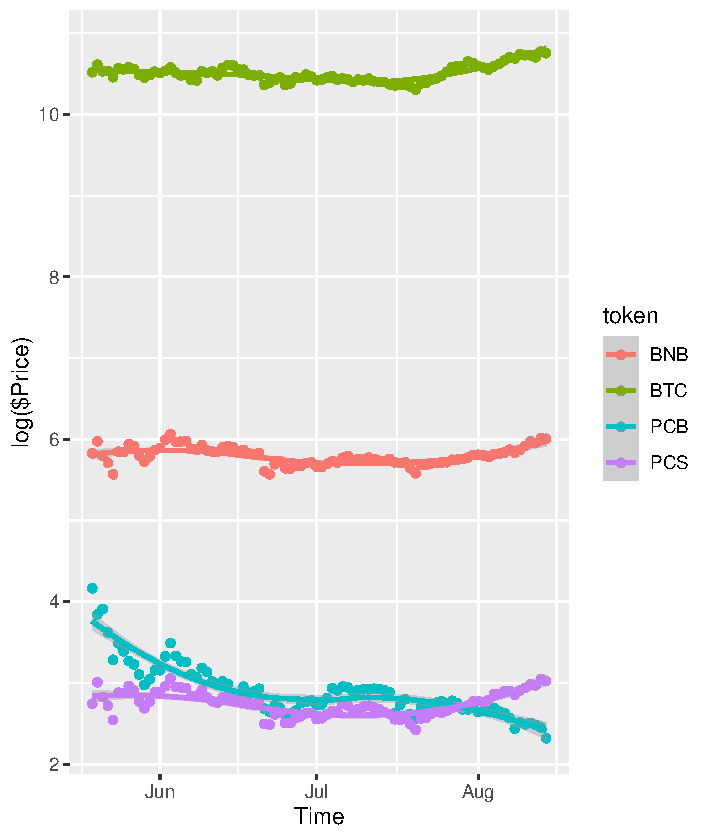
\includegraphics[height=11cm]{pcb_plot.pdf}
\caption{The three primary movers for BUNNY price are shown. The common logarithm to price of these crypto over three months (19 May – 14 August) show very distinctive features. BTC dictates the overall market sentiment, and remains stable until a small rise in the middle of July. Concomitant with BTC’s rise is an upward trend of BNB, and an even more pronounced upswing of PCS. BUNNY token, under PCB, is in a downward trend post-mortem (19 May) despite a positive market sentiment dictated by BTC and subsequently BNB. }
\end{figure}


\section*{Discussion}
PCB has initiated a massive recovery plan to expand its ecosystem with a combination of micro/macro-tokenomics, new projects, and frequent system updates. One of the most interesting projects is Qubit since it provides the L1 borrow/lending layer for Bunny. With Qubit as the foundation, PCB’s other projects are able to vertically integrate in a synergistic manner. The symbiosis becomes apparent when Single Asset Vaults (SAVs) in Bunny are able to utilize the qScore from Mound Vault’s 100M Qubits to leverage their APR \cite{bunny_qbt}. The projects that make up PCB are mutually exclusive, and collectively exhaustive — PCB aims to be free from any external third parties to deliver value. In contrast, no other competitors have announced the move to be fully vertically integrated. Whether this is a lack of engineering capacity, know-how, or vision remain unknown. The flash loan attack on PCB, although devastating (\verb|Figure 1|), ignited a spark of innovation as a clear reminder of “fate loves irony” for investors in DeFi. With this innovation in mind, there are three particular reasons why PCB is undervalued compared to its competitors:

\begin{itemize}
\item The MC/TVL of PCB is 0,13 (\verb|Table 1|) although the ecosystem is expanding aggressively. The expected MC/TVL should be ~(0,43+0,19)/2=0,31 somewhere between PCS and Beefy Finance. The MC to achieve a 0,31 MC/TVL is 0,31 x \$834,65M = \$261,53M or at least \$24/BUNNY.

\item The current TVL of PCB is nearly 10\% of the highest recorded on 3 May of almost \$8B. Most yield farms lost 20 – 50\% of their TVL since the last bull run, but Bunny should be able to double its current TVL to \$1,5B although it might take numerous months.

\item Bunny is one the most popular DeFi projects on BSC as evidenced by the number of holders, only surpassed by PCS. The number of Bunny holders even surpassed its competitors who are listed on Binance in the Innovation Zone \cite{binance_listed}.
\end{itemize}

Taken at face value, Bunny is expected to double its current TVL, establish a more balanced MC/TVL, and achieve more than  3x the current price of Bunny. The exact price of BUNNY in these conditions would be:(0,31*\$1,5B)/10,7M=\$43. This would be attainable within the next 6 – 12 months as PCB recovers, but also depends on the market although the DeFi sector on BSC grew by almost 8.000\% since January \cite{bsc_debank}. Moving forward, PCB needs to regain the trust of investors as evidenced by the low MC/TVL and TVL. Security is now the number one priority in the form of bug bounties and audits (Immunefi \cite{bunny_immunefi}, Theori \cite{bunny_theori}, Hexlant \cite{bunny_hexlant_peckshield} and Peckshield \cite{bunny_hexlant_peckshield}), testnets \cite{qbt_testnet} and proactive solutions \cite{bsc_summit}. In addition, PCB posts in-depth ( \textgreater 1000 words) Medium articles at least once a week to update their investors \cite{bunny_medium}. The writings of PCB also illustrates the delicate balance between raw talent in STEM by the developers and soft skills by the moderators. However, despite a historic compensation plan and throughout communication, investors will still have to exercise patience as time is the focus metric of trust.
PCB have leveraged every tactic to keep the ecosystem afloat. Through aggressive innovation, they have demonstrated ways to recover from one of the most severe exploits in DeFi. The current price of BUNNY is still reminiscent of its past, but over time investors' confidence may once again grow so the price of BUNNY will finally reflect the value of PCB.

\bibliography{scibib}

\bibliographystyle{Science}



\section*{Acknowledgments}
The authors are all active in Discord, and would like to thank all the members of PCB. A special thanks goes to the regular moderators: Mincus and Autolyzer. Lastly, Gerald Hefner (aka. supreme leader) and GRACKATTACK has provided valuable input to our discussions. They were truly an inspiration for this article as well as everyone else in the community.


\clearpage



\end{document}




















